% Review version (double blind). For camera-ready switch to \documentclass[cameraready]{Interspeech}
% and fill in the author block below.
\documentclass{Interspeech}
\usepackage{booktabs,amsmath,amssymb}
% Generated by experiments/make_numbers.py from results/summary.json. Do not edit.
\newcommand{\DSshortN}{1,417}
\newcommand{\DSshortSucc}{98.5}
\newcommand{\DSshortSNR}{115}
\newcommand{\DSshortMAE}{1.4\times 10^{-5}}
\newcommand{\DSshortSec}{2.5}
\newcommand{\DSshortFail}{21}
\newcommand{\DSshortFailAmb}{21}
\newcommand{\DSlongN}{191}
\newcommand{\DSlongSucc}{96.9}
\newcommand{\DSlongMAE}{4.0\times 10^{-6}}
\newcommand{\DSlongSNR}{127}
\newcommand{\DSlongSec}{37}
\newcommand{\DSlongMaxAudio}{35.0}
\newcommand{\DSlongestMAE}{1.3\times 10^{-4}}
\newcommand{\DSlongestFrames}{1,748}
\newcommand{\TFN}{600}
\newcommand{\TFSucc}{94.8}
\newcommand{\TFSNR}{63}
\newcommand{\TFSec}{8.5}
\newcommand{\TFMaxAudio}{9.6}
\newcommand{\GMmaeLo}{5.9}
\newcommand{\GMmaeHi}{8.0}
\newcommand{\GMsec}{2,973}
\newcommand{\GMn}{4}
\newcommand{\GMaudio}{2.3}
\newcommand{\AudMfccPrelimN}{39}
\newcommand{\AudMfccPrelimWEROrig}{2.2}
\newcommand{\AudMfccPrelimWERTrue}{4.0}
\newcommand{\AudMfccPrelimWERRec}{4.0}
\newcommand{\AudMfccPrelimWERGL}{6.5}
\newcommand{\AudMfccPrelimSpk}{90}
\newcommand{\AudMfccPrelimSim}{0.76}
\newcommand{\AudMfccPrelimSpeakers}{22}
\newcommand{\CkDsbegaEpbSeqSucc}{100}
\newcommand{\CkDsbegaEpbSeqSNR}{95}
\newcommand{\CkDsbegaEpbSeqN}{8}
\newcommand{\CkDsbegaLastLinearSucc}{98}
\newcommand{\CkDsbegaLastLinearSNR}{106}
\newcommand{\CkDsbegaLastLinearN}{60}
\newcommand{\CkDsbEpbaFinalbaaHLinearSucc}{98}
\newcommand{\CkDsbEpbaFinalbaaHLinearSNR}{105}
\newcommand{\CkDsbEpbaFinalbaaHLinearN}{60}
\newcommand{\CkDsbEpbaFinalbaaHSeqSucc}{100}
\newcommand{\CkDsbEpbaFinalbaaHSeqSNR}{102}
\newcommand{\CkDsbEpbaFinalbaaHSeqN}{12}
\newcommand{\CkDsbEpbLinearSucc}{98}
\newcommand{\CkDsbEpbLinearSNR}{100}
\newcommand{\CkDsbEpbLinearN}{60}
\newcommand{\CkDsbEpbSeqSucc}{100}
\newcommand{\CkDsbEpbSeqSNR}{106}
\newcommand{\CkDsbEpbSeqN}{12}
\newcommand{\CkDsbEpcLinearSucc}{98}
\newcommand{\CkDsbEpcLinearSNR}{103}
\newcommand{\CkDsbEpcLinearN}{60}
\newcommand{\CkDsbEpdLinearSucc}{98}
\newcommand{\CkDsbEpdLinearSNR}{104}
\newcommand{\CkDsbEpdLinearN}{60}
\newcommand{\CkDsbEpfLinearSucc}{98}
\newcommand{\CkDsbEpfLinearSNR}{107}
\newcommand{\CkDsbEpfLinearN}{60}
\newcommand{\CkDsbEpiLinearSucc}{98}
\newcommand{\CkDsbEpiLinearSNR}{107}
\newcommand{\CkDsbEpiLinearN}{60}
\newcommand{\CkDsbStepaLinearSucc}{98}
\newcommand{\CkDsbStepaLinearSNR}{117}
\newcommand{\CkDsbStepaLinearN}{60}
\newcommand{\CkDsbStepbaaaLinearSucc}{98}
\newcommand{\CkDsbStepbaaaLinearSNR}{102}
\newcommand{\CkDsbStepbaaaLinearN}{60}
\newcommand{\CkDsbStepbaaLinearSucc}{98}
\newcommand{\CkDsbStepbaaLinearSNR}{115}
\newcommand{\CkDsbStepbaaLinearN}{60}
\newcommand{\CkDsbStepdaaaLinearSucc}{98}
\newcommand{\CkDsbStepdaaaLinearSNR}{104}
\newcommand{\CkDsbStepdaaaLinearN}{60}
\newcommand{\CkDsbStepdaaLinearSucc}{98}
\newcommand{\CkDsbStepdaaLinearSNR}{104}
\newcommand{\CkDsbStepdaaLinearN}{60}
\newcommand{\CkTfegaLastSucc}{88}
\newcommand{\CkTfegaLastSNR}{54}
\newcommand{\CkTfegaLastN}{60}
\newcommand{\CkTfEpbSucc}{93}
\newcommand{\CkTfEpbSNR}{63}
\newcommand{\CkTfEpbN}{60}
\newcommand{\CkTfEpcgFinalbaaHSucc}{83}
\newcommand{\CkTfEpcgFinalbaaHSNR}{55}
\newcommand{\CkTfEpcgFinalbaaHN}{60}
\newcommand{\CkTfEpcgReconSucc}{91}
\newcommand{\CkTfEpcgReconSNR}{56}
\newcommand{\CkTfEpcgReconN}{80}
\newcommand{\CkTfEpfSucc}{67}
\newcommand{\CkTfEpfSNR}{52}
\newcommand{\CkTfEpfN}{27}
\newcommand{\CkTfStepaSucc}{93}
\newcommand{\CkTfStepaSNR}{64}
\newcommand{\CkTfStepaN}{60}
\newcommand{\CkTfStepdaaSucc}{90}
\newcommand{\CkTfStepdaaSNR}{63}
\newcommand{\CkTfStepdaaN}{60}
\newcommand{\CkTfStepdaaaSucc}{73}
\newcommand{\CkTfStepdaaaSNR}{48}
\newcommand{\CkTfStepdaaaN}{60}
\newcommand{\CkTfknownegaLastSucc}{93}
\newcommand{\CkTfknownegaLastSNR}{54}
\newcommand{\CkTfknownegaLastN}{60}
\newcommand{\CkTfknownEpcgFinalbaaHSucc}{90}
\newcommand{\CkTfknownEpcgFinalbaaHSNR}{55}
\newcommand{\CkTfknownEpcgFinalbaaHN}{60}
\newcommand{\CkTfknownEpfSucc}{77}
\newcommand{\CkTfknownEpfSNR}{49}
\newcommand{\CkTfknownEpfN}{60}
\newcommand{\CkTfknownStepdaaaSucc}{82}
\newcommand{\CkTfknownStepdaaaSNR}{48}
\newcommand{\CkTfknownStepdaaaN}{60}
\newcommand{\DfDsbClipaPabBlindSucc}{100}
\newcommand{\DfDsbClipaPabBlindMAE}{1.2\times 10^{-5}}
\newcommand{\DfDsbDropoutaPbLinearSucc}{98}
\newcommand{\DfDsbDropoutaPbLinearMAE}{7.5\times 10^{-6}}
\newcommand{\DfDsbDropoutaPcLinearSucc}{98}
\newcommand{\DfDsbDropoutaPcLinearMAE}{5.5\times 10^{-6}}
\newcommand{\DfDsbDropoutaPcSeqSucc}{0}
\newcommand{\DfDsbDropoutaPcSeqMAE}{7.5\times 10^{0}}
\newcommand{\DfDsbDropoutaPdLinearSucc}{98}
\newcommand{\DfDsbDropoutaPdLinearMAE}{4.0\times 10^{-6}}
\newcommand{\DfDsbDropoutaPfLinearSucc}{98}
\newcommand{\DfDsbDropoutaPfLinearMAE}{2.3\times 10^{-6}}
\newcommand{\DfDsbFbgKnownSucc}{10}
\newcommand{\DfDsbFbgKnownMAE}{2.9\times 10^{-2}}
\newcommand{\DfDsbNoisebEmbBlindSucc}{0}
\newcommand{\DfDsbNoisebEmbBlindMAE}{7.8\times 10^{0}}
\newcommand{\DfDsbNoisebEmbKnownSucc}{0}
\newcommand{\DfDsbNoisebEmbKnownMAE}{6.7\times 10^{0}}
\newcommand{\DfDsbNoisebEmcBlindSucc}{0}
\newcommand{\DfDsbNoisebEmcBlindMAE}{7.8\times 10^{0}}
\newcommand{\DfDsbNoisebEmcKnownSucc}{0}
\newcommand{\DfDsbNoisebEmcKnownMAE}{5.3\times 10^{0}}
\newcommand{\DfDsbNoisebEmdBlindSucc}{0}
\newcommand{\DfDsbNoisebEmdBlindMAE}{6.6\times 10^{-1}}
\newcommand{\DfDsbNoisebEmdKnownSucc}{0}
\newcommand{\DfDsbNoisebEmdKnownMAE}{6.6\times 10^{-1}}
\newcommand{\DfDsbNoisebEmeBlindSucc}{52}
\newcommand{\DfDsbNoisebEmeBlindMAE}{9.4\times 10^{-3}}
\newcommand{\DfDsbNoisebEmeKnownSucc}{52}
\newcommand{\DfDsbNoisebEmeKnownMAE}{9.4\times 10^{-3}}
\newcommand{\DfDsbNoisebEmfBlindSucc}{82}
\newcommand{\DfDsbNoisebEmfBlindMAE}{7.1\times 10^{-4}}
\newcommand{\DfDsbNoisebEmfKnownSucc}{82}
\newcommand{\DfDsbNoisebEmfKnownMAE}{7.1\times 10^{-4}}
\newcommand{\DfDsbNoisebEmgBlindSucc}{98}
\newcommand{\DfDsbNoisebEmgBlindMAE}{7.2\times 10^{-5}}
\newcommand{\DfDsbNoisebEmgKnownSucc}{98}
\newcommand{\DfDsbNoisebEmgKnownMAE}{7.2\times 10^{-5}}
\newcommand{\DfDsbNoisebEmhBlindSucc}{100}
\newcommand{\DfDsbNoisebEmhBlindMAE}{1.4\times 10^{-5}}
\newcommand{\DfDsbNoisebEmhKnownSucc}{100}
\newcommand{\DfDsbNoisebEmhKnownMAE}{1.4\times 10^{-5}}
\newcommand{\DfDsbPruneaPfBlindSucc}{0}
\newcommand{\DfDsbPruneaPfBlindMAE}{7.8\times 10^{0}}
\newcommand{\DfDsbPruneaPfKnownSucc}{0}
\newcommand{\DfDsbPruneaPfKnownMAE}{6.8\times 10^{0}}
\newcommand{\DfDsbPruneaPjjBlindSucc}{0}
\newcommand{\DfDsbPruneaPjjBlindMAE}{7.6\times 10^{0}}
\newcommand{\DfDsbPruneaPjjKnownSucc}{0}
\newcommand{\DfDsbPruneaPjjKnownMAE}{7.8\times 10^{0}}
\newcommand{\DfDsbPruneaPjBlindSucc}{0}
\newcommand{\DfDsbPruneaPjBlindMAE}{7.8\times 10^{0}}
\newcommand{\DfDsbPruneaPjKnownSucc}{0}
\newcommand{\DfDsbPruneaPjKnownMAE}{7.5\times 10^{0}}
\newcommand{\DfDsbQuantbgKnownSucc}{40}
\newcommand{\DfDsbQuantbgKnownMAE}{1.3\times 10^{-2}}
\newcommand{\DfDsbQuantiKnownSucc}{0}
\newcommand{\DfDsbQuantiKnownMAE}{6.1\times 10^{0}}
\newcommand{\DfDsbSignKnownSucc}{0}
\newcommand{\DfDsbSignKnownMAE}{7.6\times 10^{0}}
\newcommand{\DfDsbTrainedDropoutaPcLinearSucc}{98}
\newcommand{\DfDsbTrainedDropoutaPcLinearMAE}{2.2\times 10^{-5}}
\newcommand{\DfTfNoisebEmdKnownSucc}{0}
\newcommand{\DfTfNoisebEmdKnownMAE}{4.8\times 10^{-1}}
\newcommand{\DfTfPruneaPjKnownSucc}{0}
\newcommand{\DfTfPruneaPjKnownMAE}{8.0\times 10^{-1}}
\newcommand{\DfTfTrainmodeSucc}{95}
\newcommand{\DfTfTrainmodeMAE}{2.9\times 10^{-4}}
\newcommand{\FlLocalSgdUttsbStepsbLraPabMAE}{4.5\times 10^{-3}}
\newcommand{\FlLocalSgdUttsbStepsbLraPabSucc}{85}
\newcommand{\FlLocalSgdUttsbStepscLraPabMAE}{2.5\times 10^{-3}}
\newcommand{\FlLocalSgdUttsbStepscLraPabSucc}{90}
\newcommand{\FlLocalSgdUttsbStepsfLraPabMAE}{2.2\times 10^{-3}}
\newcommand{\FlLocalSgdUttsbStepsfLraPabSucc}{85}
\newcommand{\FlLocalSgdUttsbStepsbaLraPabMAE}{4.4\times 10^{-3}}
\newcommand{\FlLocalSgdUttsbStepsbaLraPabSucc}{100}
\newcommand{\FlLocalSgdUttsbStepsbaLraPbMAE}{2.6\times 10^{-4}}
\newcommand{\FlLocalSgdUttsbStepsbaLraPbSucc}{100}
\newcommand{\FlLocalSgdUttsbStepsfaLraPabMAE}{5.4\times 10^{-3}}
\newcommand{\FlLocalSgdUttsbStepsfaLraPabSucc}{90}
\newcommand{\FlBatchUttscStepsbLraPbMAE}{1.6\times 10^{-3}}
\newcommand{\FlBatchUttscStepsbLraPbSucc}{100}
\newcommand{\FlSgdMomentumUttsbStepsbaLraPbMAE}{1.0\times 10^{-4}}
\newcommand{\FlSgdMomentumUttsbStepsbaLraPbSucc}{95}
\newcommand{\FlSgdWeightDecayUttsbStepsbaLraPbMAE}{5.2\times 10^{-4}}
\newcommand{\FlSgdWeightDecayUttsbStepsbaLraPbSucc}{100}
\newcommand{\FlAdamUttsbStepsbLraPaabMAE}{7.4\times 10^{0}}
\newcommand{\FlAdamUttsbStepsbLraPaabSucc}{0}
\newcommand{\FlAdamUttsbStepsbaLraPaabMAE}{7.4\times 10^{0}}
\newcommand{\FlAdamUttsbStepsbaLraPaabSucc}{0}
\newcommand{\FlBatchShortUttseStepsbLraPbMAE}{5.9\times 10^{-4}}
\newcommand{\FlBatchShortUttseStepsbLraPbSucc}{90}
\newcommand{\FlBatchShortUttsiStepsbLraPbMAE}{1.3\times 10^{-3}}
\newcommand{\FlBatchShortUttsiStepsbLraPbSucc}{80}
\newcommand{\FlBatchShortUttsbgStepsbLraPbMAE}{1.1\times 10^{-3}}
\newcommand{\FlBatchShortUttsbgStepsbLraPbSucc}{85}
\newcommand{\FlLocalEpochsBatchbUttseStepsiLraPbMAE}{5.5\times 10^{-4}}
\newcommand{\FlLocalEpochsBatchbUttseStepsiLraPbSucc}{90}
\newcommand{\FlLocalEpochsBatchbUttsiStepsbgLraPbMAE}{1.1\times 10^{-3}}
\newcommand{\FlLocalEpochsBatchbUttsiStepsbgLraPbSucc}{90}
\newcommand{\CfdfbcCov}{92}
\newcommand{\CfdfbcSNR}{14}
\newcommand{\CfdfbcN}{1}
\newcommand{\CfdfbcsingleCov}{9}
\newcommand{\CfdfbcsingleSNR}{16}
\newcommand{\CfdfbcsingleN}{10}
\newcommand{\TrdsbWER}{40.7}
\newcommand{\TrdsbegaWER}{25.5}
\newcommand{\TrtfWER}{24.0}
\newcommand{\TrtfegaWER}{13.3}
\newcommand{\TrDSsucc}{98.3}
\newcommand{\TrDSwer}{41}
\newcommand{\DropSucc}{98.3}
\newcommand{\TrTFsucc}{83}
\newcommand{\TrTFknownSucc}{90}
\newcommand{\TrTFwer}{24}
\newcommand{\WERrec}{3.8}
\newcommand{\WERorig}{3.0}
\newcommand{\SpkRec}{98}
\newcommand{\Speakers}{40}
\newcommand{\PruneSucc}{0}
\newcommand{\SignSucc}{0}
\newcommand{\ConfCov}{9}
\newcommand{\ConfSNR}{16}
\newcommand{\ConfN}{10}
\newcommand{\GMmae}{5.9 to 8.0}
\newcommand{\SilencePct}{1.5}
\newcommand{\DropAllSucc}{98}
\newcommand{\WerShort}{3.8}
\newcommand{\WerOrigShort}{3.0}
\newcommand{\SpkShort}{98}
\newcommand{\SpkOrigShort}{99}
\newcommand{\AudNShort}{197}
\newcommand{\WerGLShort}{5.1}
\newcommand{\WerLong}{4.2}
\newcommand{\WerOrigLong}{3.4}
\newcommand{\SpkLong}{100}
\newcommand{\SpkOrigLong}{100}
\newcommand{\AudNLong}{57}
\newcommand{\WerTf}{4.2}
\newcommand{\WerOrigTf}{3.8}
\newcommand{\SpkTf}{99}
\newcommand{\SpkOrigTf}{99}
\newcommand{\AudNTf}{186}
\newcommand{\WerDrop}{4.7}
\newcommand{\WerOrigDrop}{2.4}
\newcommand{\SpkDrop}{98}
\newcommand{\SpkOrigDrop}{100}
\newcommand{\AudNDrop}{58}
\newcommand{\WerTfTr}{3.7}
\newcommand{\WerOrigTfTr}{2.3}
\newcommand{\SpkTfTr}{99}
\newcommand{\SpkOrigTfTr}{100}
\newcommand{\AudNTfTr}{80}


\title{Frames in the Span: Exact, Label-Free Recovery of Long-Form Speech from Federated ASR Updates}

% TODO(Taka): author list and affiliations for the camera-ready version.
\author[affiliation={1}]{Anonymous}{Author}
\address{$^1$Anonymous Institution}
\email{anonymous@example.com}
\keywords{federated learning, speech recognition, privacy, gradient inversion, CTC}

\begin{document}
\maketitle

\begin{abstract}
Federated speech recognition sends model updates to a server and keeps the audio on the device. We show
that for acoustic models whose first layer applies one linear map to overlapping windows of feature
frames, a single update contains the features. The rows of the first-layer gradient span the windows,
the overlap turns membership in that span into a linear system, and a banded solve returns the
utterance without transcript, length, loss or optimisation. The system is uniquely solvable up to
(k-s)F windows for kernel k, stride s and F features. On LibriSpeech the closed form recovers
\DSshortSucc\% of utterances up to 6.2 s from DeepSpeech and \TFSucc\% up to 9.6 s from a
Transformer-CTC front end; a sequential decoder over deeper layers reaches 35 s. Synthesised audio is
transcribed at \WerShort\% WER and the speaker identified in \SpkShort\% of cases. Local SGD, batching,
clipping, dropout and training do not prevent the attack; local Adam, pruning and sufficient noise do.
\end{abstract}

\section{Introduction}

Federated learning (FL) \cite{mcmahan2017communication} is attractive for automatic speech recognition
(ASR) because the audio stays on the device \cite{guliani2021training,nguyen2023federated,pelikan2025enabling}.
What leaves the device is a model update, and gradient inversion \cite{zhu2019dlg,geiping2020inverting}
asks how much of the input an update reveals.

For speech the evidence comes from optimisation attacks. Dang et al.\ \cite{dang2022speaker} search for
DeepSpeech \cite{hannun2014deep} input features whose gradient matches the observed one, with the
transcript and length of short utterances given, and identify the speaker in 34\% of cases; a dropout
rate of 0.2 reduces this to 0\%. Their label attack \cite{dang2021revealing} recovers bags of word
pieces. Later work matches gradients of small classifiers on one-second clips
\cite{li2023speech,ovi2024gradient}, scales to long audio by reconstructing segments of a CNN classifier's
input \cite{zeng2025recover}, or descends through the CTC loss \cite{graves2006connectionist} on
DeepSpeech \cite{bui2025reconstructing}. Speaker information also leaks from adapted weights without
reconstruction \cite{tomashenko2022privacy}. Optimisation attacks are slow, assume side information, and
fail under dropout, local training or long inputs; such failures support the view that gradient leakage
is fragile in realistic FL \cite{du2025sok,huang2021evaluating}.

A second line of work is algebraic. The gradient of a linear layer is a sum of outer products, so its
row space is the span of the layer's inputs. DAGER \cite{petrov2024dager} tests discrete tokens against
this span, SPEAR \cite{dimitrov2024spear} separates small image batches with it, and TIGER
\cite{kalikman2026tiger} optimises embeddings towards it. None of these addresses speech.

We observe that speech front ends make the span unusually easy to read. The frames of one utterance act
as a batch, and every frame is seen through a window that overlaps its neighbours: spliced context in
DeepSpeech and TDNN-style models, a strided convolution in Transformer encoders. The overlap is what
converts span membership into a linear system in the features. We contribute (i) a closed-form attack
with a capacity law verified on four front ends, (ii) a sequential decoder for utterances beyond that
capacity, (iii) an evaluation under the conditions of federated training, including trained models, and
(iv) a map of which architectures and defences stop the attack.

\section{The span leak}

\subsection{Setting}
A client holds features $X=(x_1,\dots,x_T)$, $x_t\in\mathbb{R}^F$. The first layer reads windows
$c_p(X)=[x_{ps-a},\dots,x_{ps-a+k-1}]\in\mathbb{R}^{kF}$, $p=1,\dots,P$, zero outside $1..T$, and
computes $Wc_p+b$ with $W\in\mathbb{R}^{H\times kF}$. DeepSpeech-1 splices $c$ frames of context on each
side ($k=2c+1$, $s=1$). The Transformer encoder of the FL benchmark in \cite{pelikan2025enabling} uses a
1-D convolution with $k=7$, $s=3$ on $F=80$ log-mel bins. The server is honest but curious: it knows the
model it sent and receives the update of one client.

\subsection{Span and length}
For any loss $L$ and any later layers, with $g_p=\partial L/\partial(Wc_p+b)$,
\begin{equation}
\nabla_W L=\sum_{p=1}^{P} g_p\,c_p^{\top},\qquad \nabla_b L=\sum_{p=1}^{P} g_p .
\label{eq:grad}
\end{equation}
The rows of $M=[\nabla_W L\mid\nabla_b L]$ lie in $\mathcal{S}=\mathrm{span}\{[c_p,1]\}_{p}$, and the row
space equals $\mathcal{S}$ when the $g_p$ are linearly independent. This requires $H\ge P$ and holds
generically when a nonlinearity follows. The rank of $M$ is then the number of independent windows, so
the update reveals the length of the utterance.

\subsection{Closed form and capacity}
Let $\Pi^{\perp}$ be the projector onto $\mathcal{S}^{\perp}$, from the SVD of $M$. The true features
satisfy
\begin{equation}
\Pi^{\perp}\,[c_p(X),1]=0,\qquad p=1,\dots,P .
\label{eq:lin}
\end{equation}
Each $c_p$ copies frames of $X$, so \eqref{eq:lin} is linear in $X$. Its normal matrix is block-banded
with bandwidth $kF$ and is solved by banded Cholesky in $O(TF(kF)^2)$. There are $P(kF+1-P)$ equations
for about $sPF$ unknowns, which gives the necessary condition
\begin{equation}
P\;\le\;(k-s)F+1 .
\label{eq:cap}
\end{equation}
Without overlap ($k=s$) each window may be any element of $\mathcal{S}$ and nothing is identified. The
rank fixes $P$ unless frames repeat exactly; we therefore take the shortest length whose solution lies
in the span, and test uniqueness by perturbing the solve.

\subsection{What federated training changes}
After $K$ local SGD steps the server forms $(W_0-W_K)/\eta=\sum_{j}\sum_p g_p^{(j)}c_p^{\top}$. The
windows do not depend on the weights, so the row space is unchanged. Momentum reweights the terms and
weight decay adds a known multiple of $W_0$. A batch places the windows of all its utterances in one
span, so \eqref{eq:cap} bounds the total number of frames. Norm clipping rescales $M$. Dropout after the
first layer alters $g_p$ only. Per-coordinate optimisers such as Adam destroy the structure.

\subsection{Noise}
For an update $M+E$ with i.i.d.\ Gaussian $E$ of standard deviation $\sigma$,
$\lVert E\rVert_2\approx\sigma(\sqrt{H}+\sqrt{kF+1})$ and Wedin's theorem bounds the rotation of the span by
$\rho=\lVert E\rVert_2/s_P(M)$, where $s_P$ is the weakest signal singular value. The error should grow linearly
with $\rho$ and the attack should fail near $\rho=1$.

\section{Beyond the first layer}

Past the capacity the first-layer span is the whole space. Deeper layers still leak. In DeepSpeech-1
the second and third layers and the LSTM input weights act on $h_1(c_t)$, $h_2(c_t)$, $h_3(c_t)$,
clipped-ReLU functions of a single window with 2{,}048 to 4{,}096 units. By \eqref{eq:grad} their
gradients leak $\mathcal{S}_\ell=\mathrm{span}\{[h_\ell(c_t),1]\}$, of dimension $T$ up to the layer
width. The nonlinearity is essential: a linear stack would leak the same $(kF{+}1)$-dimensional span at
every layer.

A candidate window $c$ is tested by the residual
$r(c)=\sum_\ell\lVert\Pi_\ell^{\perp}[h_\ell(c),1]\rVert^2/\lVert[h_\ell(c),1]\rVert^2$, which vanishes on the windows
of the utterance and, generically, only there. The test does not say which frame a window is, and
descending on all frames at once collapses to an average window. The zero padding provides the order.
The first window is $[0,\dots,0,x_1,\dots,x_{c+1}]$; we solve for it by Levenberg--Marquardt from the
opening frames of public utterances. Each later window shares all frames but one with its predecessor,
leaving $F$ unknowns per step. We use the spans of the second and third layers; the LSTM-input span is noisier on trained weights and is
needed only beyond 37\,s. The last 26 frames are re-fitted jointly every 8 steps, which keeps the
recursion from drifting. Decoding stops when $c$ consecutive frames are zero: the
padding at the far end. The length is thus an output. A joint refinement of all frames follows.

The same idea applies to any front end whose features are local in time. For Conv2dSubsampling followed
by a linear projection \cite{gulati2020conformer}, the projection leaks the span of 7-frame receptive
fields, and a decoder can seed on any window and extend in both directions.

\section{Experiments}

\subsection{Setup}
Data: LibriSpeech \cite{panayotov2015librispeech} test-clean; one float32 gradient of the CTC loss per
utterance. \textbf{DeepSpeech-1}: 26 MFCCs at 50\,Hz, $c=6$, three clipped-ReLU layers of 2{,}048
(4{,}096) units, a BiLSTM, two output layers. \textbf{Transformer-CTC}: 80 log-mel bins at 100\,Hz,
per-utterance normalisation, Conv1d$(80{\to}1536)$ with $k{=}7$, $s{=}3$ and a gated linear unit, 12
pre-norm blocks of width 768. Both are attacked at random initialisation and along training on
train-clean-100. The attacker receives the update and the model. Public data (train-clean-100, disjoint
speakers) supplies starting points and trains the vocoder front end. An utterance counts as recovered if
its mean absolute error (MAE) is below $10^{-2}$ for MFCCs, whose mean magnitude is 8, or if its SNR
exceeds 30\,dB for normalised log-mel.

\begin{table}[t]
\caption{One update per utterance. SNR is the median over utterances of the feature-domain SNR.
$^\dagger$length given (\TrTFsucc\% without). $^\ddagger$transcript and length given.}
\label{tab:main}
\centering\footnotesize
\setlength{\tabcolsep}{3pt}
\begin{tabular}{@{}llrrr@{}}
\toprule
Target & Attack & $n$ & Recov. & SNR\\
\midrule
DS1, $\le$6.2\,s & closed form & \DSshortN & \DSshortSucc\% & \DSshortSNR\\
DS1, 6.3--\DSlongMaxAudio\,s & sequential & \DSlongN & \DSlongSucc\% & \DSlongSNR\\
DS1 trained & closed form & 60 & \TrDSsucc\% & \\
DS1 trained, dropout 0.2 & closed form & 60 & \DropSucc\% & \\
Transf., $\le$9.6\,s & closed form & \TFN & \TFSucc\% & \TFSNR\\
Transf.\ trained & closed form$^\dagger$ & 60 & \TrTFknownSucc\% & \\
Gradient matching$^\ddagger$ \cite{bui2025reconstructing} & 2{,}000 steps & \GMn & 0\% & $<$3\\
\bottomrule
\end{tabular}
\end{table}

\begin{figure}[t]
\centering
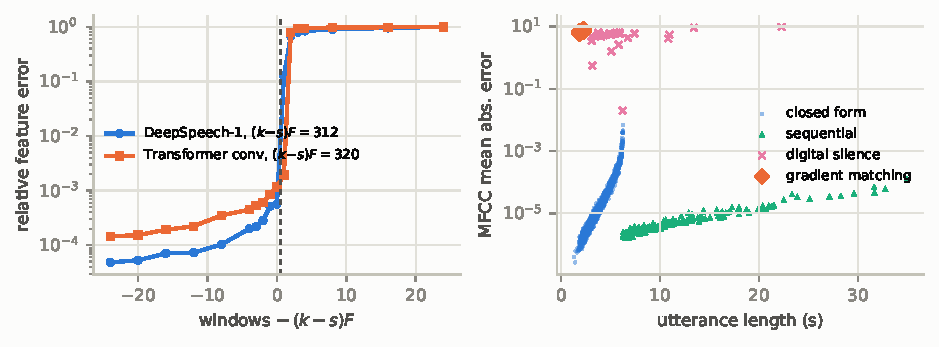
\includegraphics[width=\linewidth]{../../docs/figures/paper_main.pdf}
\caption{Left: relative error of the closed form around the predicted capacity. Right: MAE against
utterance length for all attacked utterances.}
\label{fig:main}
\end{figure}

\subsection{Closed form}
On DeepSpeech-1 the closed form recovers \DSshortSucc\% of the \DSshortN{} test-clean utterances that
fit in the first layer (Table~\ref{tab:main}), with median MAE $\DSshortMAE$ in \DSshortSec\,s, and
reads the length from the rank (Fig.~\ref{fig:spectrum}). All \DSshortFail{} failures are flagged by the uniqueness test: the
recordings contain runs of bit-identical frames (digital silence) that make windows identical. On the
Transformer front end, \TFSucc\% of \TFN{} utterances up to 9.6\,s are recovered at \TFSNR\,dB.
Fig.~\ref{fig:main} (left) crops real features to exact lengths: the error stays below $10^{-3}$ up to
$(k-s)F$ windows and reaches order one within two windows, for $(k,s,F)=(13,1,26)$, $(19,1,26)$,
$(7,3,80)$ and $(5,2,80)$.

\subsection{Long-form speech}
The sequential decoder recovers \DSlongSucc\% of \DSlongN{} utterances between 6.3 and
\DSlongMaxAudio\,s, with median MAE $\DSlongMAE$, including the longest utterance of the set
(\DSlongestFrames{} frames). The remaining failures are digital silence. Decoding takes \DSlongSec\,s per utterance
(median, one GPU) and involves neither the LSTM nor the loss. Checkpoints trained to \TrDSwer\% WER are decoded equally well
(12 of 12 utterances).

\subsection{Comparison with gradient matching}
We rerun output-layer gradient matching through a twice-differentiable CTC with transcript and length
given. After 2{,}000 Adam steps (\GMsec\,s) on 2\,s utterances the cosine distance is below $10^{-2}$
and the MAE is \GMmae: the output-layer gradient has rank at most 29 and cannot determine hundreds of
frames. Matching all layers exceeded 34\,GB of GPU memory at 100 frames.

\begin{figure*}[t]
\centering
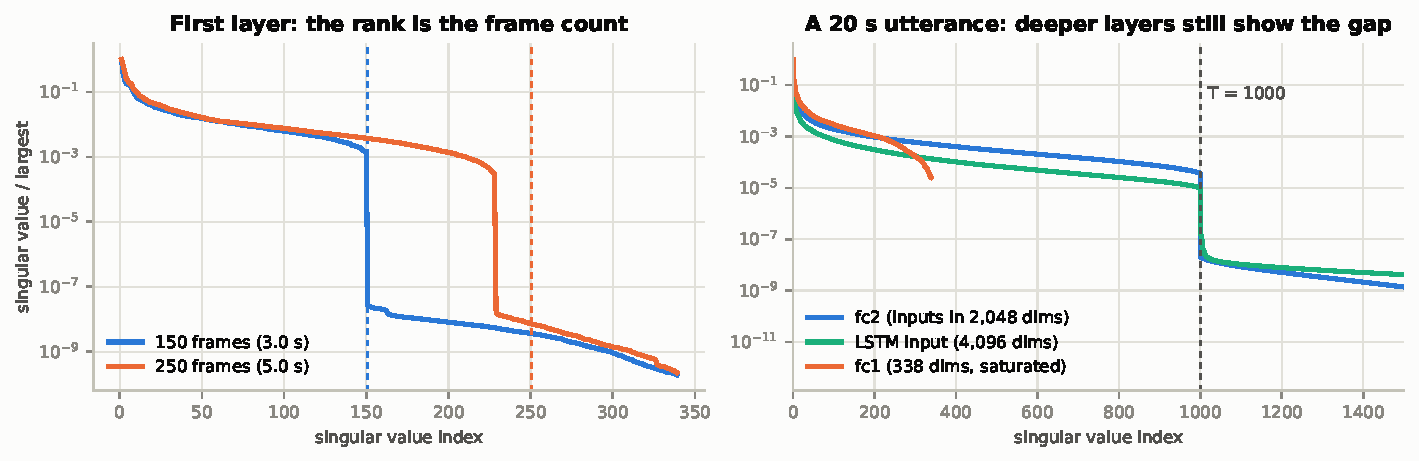
\includegraphics[width=0.86\textwidth]{../../docs/figures/spectrum.pdf}
\caption{Singular values of gradients from DeepSpeech-1, relative to the largest. Left: first layer, two
short utterances; the spectrum drops to the float32 floor exactly at the frame count. Right: a 20\,s
utterance saturates the first layer, but the second layer and the LSTM input weights still show the gap.}
\label{fig:spectrum}
\end{figure*}

\begin{table}[t]
\caption{Closed form on the first-layer update of DeepSpeech-1 under federated conditions (top, 20 trials
each, update formed from float32 weight differences) and defences (bottom, 40 to 60 utterances each).
Recovered: MAE below 0.1 (top), below 0.01 (bottom).}
\label{tab:fl}
\centering\footnotesize
\begin{tabular}{@{}lrr@{}}
\toprule
Condition & Median MAE & Recov.\ (\%)\\
\midrule
1 SGD step & $4.5\cdot10^{-3}$ & 85\\
10 SGD steps & $4.4\cdot10^{-3}$ & 100\\
50 SGD steps & $5.4\cdot10^{-3}$ & 90\\
SGD, momentum 0.9 & $1.0\cdot10^{-4}$ & 95\\
SGD, weight decay & $5.2\cdot10^{-4}$ & 100\\
batch of 2 & $1.6\cdot10^{-3}$ & 100\\
batch of 8 (short) & $1.3\cdot10^{-3}$ & 80\\
batch of 16 (short) & $1.1\cdot10^{-3}$ & 85\\
10 Adam steps & $7.4\cdot10^{0}$ & 0\\
\midrule
dropout 0.2 & $5.5\cdot10^{-6}$ & 98\\
dropout 0.5 & $2.3\cdot10^{-6}$ & 98\\
clipping to 0.01 & $1.2\cdot10^{-5}$ & 100\\
noise $10^{-5}$ of RMS & $7.1\cdot10^{-4}$ & 82\\
noise $10^{-3}$ of RMS & $6.6\cdot10^{-1}$ & 0\\
8-bit quantisation & $6.1\cdot10^{0}$ & 0\\
prune 50\% & $6.8\cdot10^{0}$ & 0\\
sign only & $7.6\cdot10^{0}$ & 0\\
\bottomrule
\end{tabular}

\end{table}

\subsection{Federated conditions and training}
Table~\ref{tab:fl} forms the update from float32 weight differences. The closed form is unaffected by 1
to 50 local SGD steps, momentum 0.9 and weight decay (median MAE $10^{-4}$ to $6\cdot10^{-3}$; the floor
is rounding in the subtraction and falls with larger steps). Batches of 2 to 16 utterances within
capacity are recovered when the attacker knows their lengths; a batch over capacity is not. Dropout rates from 0.1 to 0.5 leave \DropAllSucc\% recovered, in contrast
with the protection reported against optimisation attacks \cite{dang2022speaker}. DeepSpeech-1
checkpoints from initialisation to \TrDSwer\% WER are recovered at \TrDSsucc\%. On the trained
Transformer a float32 convolution artefact lies close to the weakest signal direction and the window
count is sometimes off by one; with the length given, \TrTFknownSucc\% are recovered.

\subsection{From features to audio}
A 6-layer Transformer maps recovered features to the mel input of a public HiFi-GAN
\cite{kong2020hifigan}. Whisper small.en \cite{radford2023robust} transcribes the audio and ECAPA-TDNN
embeddings \cite{desplanques2020ecapa} assign it to one of \Speakers{} enrolled test speakers
(Table~\ref{tab:audio}). Since recovery is exact, audio from recovered and from true features scores the
same: what the front end keeps, the update gives away.

\begin{table}[t]
\caption{Audio synthesised from recovered features: Whisper WER and speaker identification top-1.}
\label{tab:audio}
\centering\footnotesize
\setlength{\tabcolsep}{3pt}
\begin{tabular}{@{}lrrrrr@{}}
\toprule
 & & \multicolumn{2}{c}{WER (\%)} & \multicolumn{2}{c}{Speaker (\%)}\\
Reconstructions & $n$ & orig. & recov. & orig. & recov.\\
\midrule
DS1, $\le$6.2\,s & \AudNShort & \WerOrigShort & \WerShort & \SpkOrigShort & \SpkShort\\
DS1, 6.3--35\,s & \AudNLong & \WerOrigLong & \WerLong & \SpkOrigLong & \SpkLong\\
Transformer, $\le$9.6\,s & \AudNTf & \WerOrigTf & \WerTf & \SpkOrigTf & \SpkTf\\
\bottomrule
\end{tabular}
\end{table}

\subsection{What stops the attack}
Local Adam, magnitude pruning of half the entries and sign compression break the low-rank structure
(0\% recovered). Gaussian noise behaves as predicted: the relative error equals about $0.5\rho$ up to
$\rho\approx0.3$, and the attack fails near $\rho=1$, a noise level near $10^{-3}$ of the gradient RMS
for utterances of a few seconds. Central differential privacy adds noise after aggregation and does not
protect a client from the server.

\begin{table}[t]
\caption{Gradient rank of early layers on one 5\,s utterance (Whisper and wav2vec 2.0 with released
weights). A layer leaks a usable span when the rank equals the number of windows and is below both of its
dimensions.}
\label{tab:probe}
\centering\footnotesize
\setlength{\tabcolsep}{3pt}
\begin{tabular}{@{}llrrl@{}}
\toprule
Model & Layer & Windows & Rank & Leaks\\
\midrule
wav2vec 2.0 & first conv & 15999 & 10/10 & no\\
wav2vec 2.0 & feature proj. & 249 & 249/512 & yes\\
Whisper & conv1 & 3000 & 241/241 & no\\
DeepSpeech-1 & fc1 & 250 & 250/339 & yes\\
Transf.-CTC & conv & 166 & 167/561 & yes\\
DeepSpeech-2 & first conv & 20331 & 32/32 & no\\
DeepSpeech-2 & RNN input & 251 & 242/800 & no\\
QuartzNet & depthwise conv & 249 & 33/33 & no\\
QuartzNet & pointwise conv & 249 & 65/65 & no\\
Conformer & first conv & -- & 10/10 & no\\
Conformer & proj. after subs. & 123 & 123/256 & yes\\
\bottomrule
\end{tabular}

\end{table}

Architecture matters most (Table~\ref{tab:probe}). The first layers of pretrained Whisper (inputs padded to 3{,}000 frames) and wav2vec
2.0 \cite{baevski2020wav2vec} (10-sample windows), of DeepSpeech-2 \cite{amodei2015deep} (32 channels)
and of QuartzNet \cite{kriman2020quartznet} (depthwise) are saturated and leak no usable span. The
wav2vec 2.0 feature projection and the projection after Conformer subsampling have rank equal to the
frame count; on the latter our local decoder finds true windows but recovers only \ConfCov\% of the frames on average
(\ConfSNR\,dB) before its chains stall, which we count as a negative result for now. Dropout stops the
sequential decoder as well, since deeper layers see the dropped activations; it does not stop the closed form.

\section{Conclusion}

A wide linear layer over overlapping feature windows makes one federated update equivalent to the
utterance, up to a capacity we can state in advance. Dropout, clipping, local SGD and training do not
change this; breaking the low-rank structure or exceeding the capacity does. Limitations: the attack
recovers features, and pitch in the audio is inferred by the vocoder; digital silence makes solutions
non-unique; updates aggregated over many clients exceed the capacity. Code, per-utterance results and
audio are in the supplementary material.

\section{Generative AI Use Disclosure}
% TODO(Taka): this section must describe the actual use and comply with the Interspeech policy before submission.
A generative AI coding assistant was used to implement and run experiments and to draft this manuscript
from the experimental results. The authors are responsible for the content and must revise the text
before submission so that it complies with the Interspeech policy on generative AI.

\bibliographystyle{IEEEtran}
\bibliography{../refs}

\end{document}
